\documentclass{beamer}

\usepackage[brazil]{babel}
\usepackage[utf8]{inputenc}
\usepackage[T1]{fontenc}
\usepackage{listings}
\usepackage{textcomp}

\usetheme{Madrid}
\setbeamertemplate{navigation symbols}{}

\lstset{
language=Python,
upquote=true,
basicstyle=\ttfamily\tiny,
backgroundcolor=\color{white},
keywordstyle=\color{blue}\bfseries,
stringstyle=\color{red},
commentstyle=\color{green},
%morecomment=[s][\color{green}]{/**}{*/},
showspaces=false,
showstringspaces=false,
morekeywords={None,self,__init__,True,False},
literate=
{á}{{\'a}}1
{Á}{{\'A}}1
{à}{{\`a}}1 
{À}{{\`A}}1
{â}{{\^a}}1 
{Â}{{\^A}}1
{ã}{{\~a}}1
{Ã}{{\~A}}1
{ä}{{\"a}}1
{Ä}{{\"A}}1
{é}{{\'e}}1
{É}{{\'E}}1
{è}{{\`e}}1
{È}{{\`E}}1
{ê}{{\^e}}1
{Ê}{{\^E}}1
{ẽ}{{\~e}}1
{Ẽ}{{\~E}}1 
{ë}{{\"e}}1
{Ë}{{\"E}}1
{í}{{\'i}}1
{Í}{{\'I}}1
{ì}{{\`i}}1
{Ì}{{\`I}}1
{î}{{\^i}}1
{Î}{{\^I}}1
{ĩ}{{\~i}}1
{Ĩ}{{\~I}}1
{ï}{{\"i}}1
{Ï}{{\"I}}1
{ó}{{\'o}}1
{Ó}{{\'O}}1
{ò}{{\`o}}1
{Ò}{{\`O}}1
{ô}{{\^o}}1
{Ô}{{\^O}}1
{õ}{{\~o}}1
{Õ}{{\~O}}1
{ö}{{\"o}}1
{Ö}{{\"O}}1
{ú}{{\'u}}1
{Ú}{{\'U}}1
{ù}{{\`u}}1
{Ù}{{\`U}}1
{û}{{\^u}}1
{Û}{{\^U}}1
{ũ}{{\~u}}1
{Ũ}{{\~U}}1
{ü}{{\"u}}1
{Ü}{{\"U}}1
{ç}{{\c{c}}}1
{Ç}{{\c{C}}}1
}

\title[Fundamentos de Programação]{Fundamentos de Programação}

\author[Diego S. C. Nascimento]{Diego Silveira Costa Nascimento}

\institute[IFRN]{
Instituto Federal de Educação, Ciência e Tecnologia do Rio Grande do Norte\\
diego.nascimento@ifrn.edu.br
}

\date[\today]{\today}

\begin{document}

\begin{frame}[plain]
	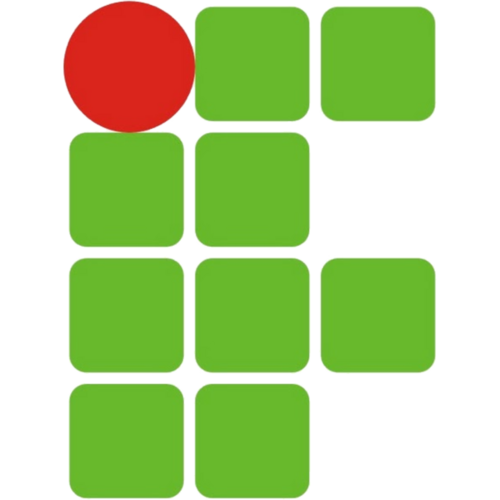
\includegraphics[scale=0.2]{img/IFRN}
	\titlepage
\end{frame}

\logo{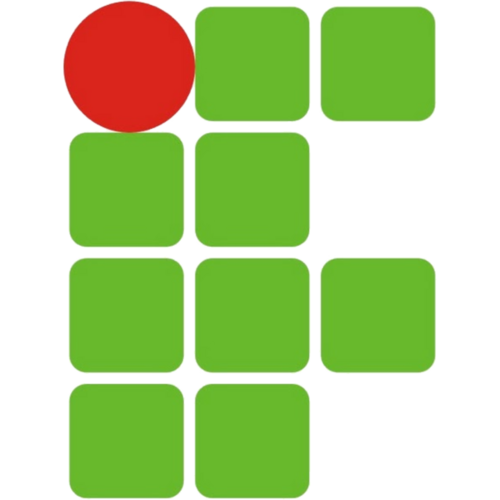
\includegraphics[scale=0.1]{img/IFRN}}

\begin{frame}
	\frametitle{Ementa do Curso}
  	\tableofcontents
\end{frame}

\AtBeginSection[]{
	\begin{frame}
		\frametitle{Ementa do Curso}
		\tableofcontents[currentsection]
	\end{frame}
}

\section{Introdução}

\begin{frame}
	\frametitle{Python}

	\begin{block}{Definição}
		É uma linguagem de script de propósito geral, podendo ser usada para criar
		qualquer tipo de software.
	\end{block}\vfill
	
	\begin{itemize}
		\item Foi concebido no final de 1989 por Guido van Rossum; e
		\item O nome Python teve a sua origem no grupo humorístico britânico
		Monty Python.
	\end{itemize}
\end{frame}

\begin{frame}
\frametitle{Características}

\begin{itemize}
	\item É uma linguagem interpretada;
	\item Os tipos das variáveis são determinados dinamicamente;
	\item Oferece tipos de alto nível;
	\item É orientada a objetos; e
	\item É multi-plataforma.
\end{itemize}
\end{frame}

\begin{frame}
\frametitle{Programa em Python}

\begin{itemize}
	\item Um programa em Python pode ser escrito em qualquer editor de texto;
	\item O documento com o código fonte deve ser salvo com extensão .py;
	\item Para facilitar o desenvolvimento é comum utilizar-se um IDE
	(Integrated Development Environment); e
	\item O IDLE é o ambiente de desenvelvimento padrão.
\end{itemize}
\end{frame}

\section{Estrutura}

\begin{frame}[fragile]
\frametitle{Instrução de Saída}

\begin{block}{Definição}
	A instrução de saída de dados é a instrução através da qual o computador se comunica com usuário durante a execução do programa. Isso é feito, geralmente, através da exibição de alguma informação na tela.
\end{block}\vfill

\begin{itemize}
	\item Em Python existe apenas um comando para instrução de saída: \structure{print}.
\end{itemize}\vfill

\begin{exampleblock}{Exemplo}
\begin{lstlisting}
print('Oi, mundo!')
\end{lstlisting}
\end{exampleblock}
\end{frame}

\begin{frame}[fragile]
\frametitle{Comentário}

\begin{block}{Definição}
É uma estrutura da linguagem que permite ao desenvolvedor fazer uma breve explicação do código escrito.
\end{block}\vfill

\begin{itemize}
	\item Comentários são iniciados com \#.
\end{itemize}\vfill

\begin{exampleblock}{Exemplo}
	\begin{lstlisting}
# Descrição da funcionalidade desenvolvida
# Autor : Diego
print ('Testando!')
	\end{lstlisting}
\end{exampleblock}\vfill

\begin{alertblock}{Importante}
O que for escrito no bloco de comentário será ignorado pelo interpretador.
\end{alertblock}
\end{frame}

\section{Variável}

\begin{frame}
\frametitle{Variável}

\begin{itemize}
	\item Uma variável representa uma posição de memória;
	\item Possui um nome e tipo;
	\item Seu conteúdo pode variar ao longo do tempo, durante a execução do
	programa;
	\item Embora uma variável possa assumir diferentes valores, ela só pode
	armazenar um valor a cada instante;
	\item Não existe limite para o número de variáveis em um programa; e
	\item Cada variável criada ocupa um espaço de memória de acordo com seu
	tipo e seu tamanho.
\end{itemize}

\end{frame}

\begin{frame}
\frametitle{Declaração de Variável}

\begin{itemize}
	\item A tipagem de Python é dinâmica;
	\item Logo não é necessário declarar os tipos de variáveis;
	\item Devem ser declaradas inicialmente por letras $(a - z, A - Z)$ ou sublinhado (\_);
	\item Acentuação é permitida (\alert{não é recomendado}); e
	\item É case sensitive $(a \neq A)$.
\end{itemize}\vfill

\begin{exampleblock}{Exemplos}
\begin{columns}[c] 
	\column{.4\textwidth}
	i\\
	nome\\
	data\_nascimento
	
	\column{.5\textwidth}
	nota1\\
	\_sexo\\
	mediaGeral
\end{columns}
\end{exampleblock}
\end{frame}

\begin{frame}[fragile]
\frametitle{Tipos de Variável}

\begin{itemize}
	\item \structure{str} : Cadeia de caracteres;
	\item \structure{int} : Inteiro;
	\item \structure{float} : Ponto flutuante ou real; e
	\item \structure{bool} : Lógico ou booleano.
\end{itemize}\vfill

\begin{exampleblock}{Exemplos}
\begin{lstlisting}
type('Python')
type(36)
type(82.5)
type(True)
\end{lstlisting}
\end{exampleblock}
\end{frame}

\end{document}